\ifsvnmulti
 \svnkwsave{$RepoFile: lyapunov/students.tex $}
 \svnidlong {$HeadURL$}
 {$LastChangedDate$}
 {$LastChangedRevision$} {$LastChangedBy$}
 \svnid{$Id$}
\fi

\chapter{Students log}
\label{c-students}

\section{Qi Ge's project}
\label{sect:introQG}
This section is an evolving draft of the introduction to Qi Ge's project.

Predrag's vision of what the project is sketched in \refchap{c-draft}. Studying
\refchap{s:LyapunovVec} is also a good idea.
Search for\\
``2012-02-06 Evangelos Talked with Hugues at MPIPKS, created a to-do list:''
\\
to see Evangelos and Hugues concrete work plan.

We hope that Qi Ge masters computation of covariant Lyapunov vectors for
the \po s and \rpo s in our \KS\ database.

\refChap{sect:LyapKS} deals specifically with the \KS\ calculations.

\subsection{\KSe}

\PC{2013-03-19 Predrag copied this from \refref{SCD07}, to set up
the conventions for which version of \KSe\ is being used}
%
In the formulation
adopted here, the time evolution of the `flame front velocity'
$u=u(x,t)$ on a periodic domain $u(x,t) = u(x+L,t)$ is given by
\beq
  u_t = F(u) = -{\textstyle\frac{1}{2}}(u^2)_x-u_{xx}-u_{xxxx}
    \,,\qquad   x \in [-L/2,L/2]
    \,.
\ee{ks}
Here $t \geq 0$ is the time, and $x$ is the spatial coordinate.
The subscripts $x$ and $t$ denote partial derivatives with respect to
$x$ and $t$. In what follows
we shall state results of all calculations either in units of the
`dimensionless system size' $\tildeL$, or the system size $L = 2 \pi
\tildeL$. All numerical results presented in this paper
are for the system size $\tildeL=22/2\pi = 3.5014\ldots$.
Spatial periodicity $u(x,t)=u(x+L,t)$
makes it convenient to work in the Fourier space,
\beq
  u(x,t)=\sum_{k=-\infty}^{+\infty} a_k (t) e^{ i k x /\tildeL }
\,,
\ee{eq:ksexp}
with the $1$-dimensional PDE \refeq{ks}
replaced by an infinite set of
ODEs for the complex Fourier coefficients $a_k(t)$:
\beq
\dot{a}_k= \pVeloc_k(a)
     = ( q_k^2 - q_k^4 )\, a_k
    - i \frac{q_k}{2} \sum_{m=-\infty}^{+\infty} a_m a_{k-m}
\,,
\ee{expan}
where $q_k = k/\tildeL$.
Since $u(x,t)$ is real, $a_k=a_{-k}^\ast$, and we can replace the
sum by a $k > 0$ sum.



\section{Daily log}

This section is the daily (or at least, bi-weekly)  log of the students'
work.

\refChap{sect:LyapKS} deals specifically with the \KS\ calculations.


\begin{description}

\item[2013-01-11 Predrag] Qi Ge  <intertwistlet@gmail.com> joined the
collaboration as a research project student (GaTech credit 3 h/week).
He will enter notes on his day-to-day progress into this log.

\item[2013-01-12 Kazumasa]
Great! Please recommend Ge Qi to read, apart from books and reviews on
chaos and orbit expansion (Chaosbook and Eckmann-Ruelle review?),
Francesco et al.'s
\HREF{http://prl.aps.org/abstract/PRL/v99/i13/e130601}{PRL}\rf{ginelli-2007-99}, and their
\HREF{http://arxiv.org/abs/1212.3961}{long follow-up paper}\rf{GiChLiPo12}.

Otherwise he wouldn't understand anything on the codes (and the project).

Hugues will stay in Japan for 2 weeks in late February. I hope that you,
the student, and Evangelos will also have time to join the discussions
during this period.

\item[2013-01-12 Qi Ge]
Great, this will be a good start point.

\item[2013-01-23 Predrag] Please ask Jeffrey M. Heninger
<jeffrey.heninger@gatech.edu> to help you get started with this
subversion repository (come to me or skype me if there is something you
cannot do):

\texttt{svn://zero.physics.gatech.edu/siminos}

user: geqi  password: Lyapunov

\item[2013-02-14 Qi Ge 2 Kazumasa]
Can you send me the code about computing the CVLs of the KS system?
So what algorithms you use in the time step simulation, this will
help me understand the code.

\item[2013-02-14 Predrag to Qi Ge] If you look into directory
siminos/chaos/ and pdflatex blog.tex, you can see an example of what
a student work log looks like (after a semester of so of work). Chao
Shi stopped with daily / weekly updates, and I ended up writing all
of Chapter 1 {\em Kuramoto-Sivashinsky equation}, so we stopped the
project.

\item[2013-02-14 Predrag to Qi Ge] Please start writing down the
ideas we talked about today into \refsect{sect:introQG}; this will
be a continuously evolving draft of the introduction to the project
report. I have entered pointers to Evangelos, Hugues and my ideas
about what the project. If we know where are you in the project, we can
help you.

\item[2013-02-14 Kazumasa to Qi Ge]
Please find my code in C++ and README at siminos/kazz/code/.
You can compile and run it as usual C++ program.
Note that, though I extracted a part of my long code relevant to our project,
 it contains many functions which are hardly used in the usual situation.

In any case, we (Hugues and myself) (Predrag: I agree, totally)
strongly recommend that you write your own code from zero, with
reference to mine. This is the best way to learn what's going on in
the code. Don't try to write a code with full functionality from the
beginning, but start with a minimal code, which only computes, say,
Lyapunov exponents.
Confirming this works as you expect, you can add a code to compute
the covariant vectors from a simple forward-backward process (and
check if the exponents values computed from the covariant vectors
agree with those from the Gram-Schmidt method). For practical use,
you have to implement the "block-by-block" computation of the
vectors, to overcome memory issues (see discussions in Sec. 4.2 in F.
Ginelli \textit{et al.}, \arXiv{1212.3961}\rf{GiChLiPo12}). This is
the first step you should reach in this project.

\item[2013-02-14 Kazumasa to Qi Ge]
For numerical integration of the KS equation, I used the
operator-splitting algorithm (Adams-Moulton method + Heun's method),
typically with time step 0.005.
For more detail, look at Sec. II A in K. A. Takeuchi \textit{et al.},
 Phys. Rev. E \textbf{84}, 046214 (2011)\rf{TaGiCh11}.

\item[2013-02-16 Qi Ge to Predrag] So our aim is to calculate the
first seven CLVs of KS system. The solution of the equation we choose
are the hyperbolic periodic orbits.

\item[2013-02-16 Predrag] Our first goal is to learn
how to compute \emph{all} eigenvectors (CLVs) and Floquet multipliers
(mistakenly often called `Lyapunov exponents' in this text) of
\JacobianM s for \po s computed in \refref{SCD07}. For \KS\
calculations of \refchap{sect:LyapKS}, system size $L=22$, this is 62
eigenvectors. We have at least 40,000 \rpo s. You will first check
whether you agree with Kazumasa's results for his favorite orbit
favorite cycle \PO{10.25}, then the new work starts.

You will have to switch from the tweets to writing up full fledged
derivations and explanations of what you are learning - clear enough
that some of that text can be later used in your term report, or a
publication, if we get that far. Clear exposition is 1/3 of research.

\item[2013-02-22 Predrag to Qi Ge] Eight weeks of the Spring semester
are gone, and I have no way of knowing whether you have done anything
at all on the project. You have not written anything substantial
following our discussion, and the request  of {\bf [2013-02-14
Predrag to Qi Ge]}. Either you work on the project, or you do not -
anything else is waste of Kazumasa's, Evangelos and my time.

If you do not write a log of what you have learned / done this week,
the next week we will discuss finding another project adviser for
you. Last warning.

\item[2013-02-22 Qi Ge] So sorry for not writing a log. I have just
finished the C++ program to calculate the Lyapunov exponents of the
\KS\ system. The code \texttt{lya\_exp.cpp} is in the
\texttt{siminos/ge/cpp/} folder. The program is running relatively
slowly. I wish to confirm the result in \refref{SCD07},
\HREF{http://www.cns.gatech.edu/~predrag/papers/SCD07.pdf}{sect. 4}:
    \PC{the source file is in \texttt{siminos/rpo\_ks/}}

\begin{quote}
``[...] Indeed, numerically the covariant Lyapunov
vectors\rf{ginelli-2007-99} of the $L=22$ chaotic attractor separate
into 8 ``physical'' vectors with small Lyapunov exponents
$(\Lyap_j) = (0.048,$ 0, 0, $-0.003$, $-0.189$, $-0.256$,
$-0.290$, $-0.310$),
and the remaining 54 ``hyperbolically isolated'' vectors with rapidly
decreasing exponents
$(\Lyap_j) = (-1.963$,   $-1.967$,   $-5.605$,   $-5.605$,  $-11.923$,  $-11.923$,
 $\cdots) \approx -(j/\tildeL)^4$,
in full agreement with the Yang \etal\rf{YaTaGiChRa08} investigations
of KS for large systems sizes.
 [...]''
\end{quote}

    Here is my choice of the parameters:
    The cutoff of k is 127 and timestep is 0.001. I plan to run the
    simulation in 1000 steps. I have not yet added any
    verification to whether this should stop there or earlier or
    later. The integration algorithm is 4th-order Runge-Kutta.

\item[2013-02-22 Predrag] To help a bit with starting writing, I have
edited your text (you can see edits by using diff in Tortoise).

You entry is way to cryptic. {\color{red} Write down here}, in your
log, the equations you are integrating (you can clip and paste
equations from elsewhere in this repository to save time). When you
write up the project report it will all be needed, so you might just
as well do it now. Let me see the real write up by this weekend
(unless you have some pressing priorities, like midterms, in your
courses).

Did you write the code from scratch, or did you get parts of it from
somewhere? I agree with Kazumasa: you want to write your own code,
but not necessarily reinvent the wheel. There is KS code various
places in this svn repository, for example in
\texttt{siminos/matlab/}, that you might want to compare performance
of your code with. Evangelos can help you with that.

\item[2013-03-02 Qi Ge] So far I have attempted to compute sets of Lyapunov
exponents for L=22 and L=96 \KS. But I am worried about the results I
get. I will first explain my algorithms below to see if it they right.

\item[2013-03-02 Qi Ge]
I integrate the \KS\ equations in Fourier representation \refeq{expan}.
    \PC{Please read any of the papers on \KS; I do not think anybody
    has $m=-N, -N-1, \cdots, -2,-1$ terms in their calculations - they
    can be eliminated by the reality of $u(x,t)$.}
\beq
\dot{a}_k=(q_{k}^2-q_{k}^4)a_k-i\frac{q_k}{2}\sum_{m=-N}^{m=N}a_{m}a_{k-m}
\ee{QGe:KS}
Here I set a the Fourier modes truncation cutoff $N$. As $k$
becomes larger, $a_k$'s converge to zero very fast. So I drop
$a_k$ terms when $k>N$. Anyway, I ignored the methods described in
\HREF{http://www.cns.gatech.edu/~predrag/papers/SCD07.pdf}
{Appendix A} of \refref{SCD07}.
    \PC{Why? The authors have lots of experience and they went to the
    trouble of explaining the best methods they know, so why not read
    them and implement them?}

Then I define a set of basis. For example: (choosing $N = 64$)
$(\varPsi_{-63},\varPsi_{-62},...\varPsi_{63})$, I can set the
initial value for the basis like $\varPsi_i=(0,...0,i,0,...,0)$.
    \PC{what is the relation of $\varPsi_i$ to ${a}_k$ of
    \refeq{expan}? Or is it the tangent space basis? Is it Fourier
    modes, is it orthogonal, does it stay orthogonal, or what?
    Describe {\color{red}in detail} the theory, definitions \etc\
    that you use - it all goes into your project report,
    \refsect{sect:introQG}, which at the moment (8 weeks into the
    semester) has {\color{red} nothing} in it.}
    %
    \PC{Why start with $\varPsi_k=(0,\cdots,0,k,0,\cdots,0)$? Should
    these be normalized, $\norm{\varPsi}=1$? Why set large, most
    unphysical components to the largest values of $k$? Probably does
    not matter for asymptotic times...}

Then I integrate numerically the ``basis set'' using the 4-th order
explicit Runge-Kutta integration routine, and the method described in
depth in the Ginelli \etal\
%\HREF{http://prl.aps.org/pdf/PRL/v99/i13/e130601}
{description of the algorithm}\rf{GiChLiPo12}
    \PC{Have you studied \refref{GiChLiPo12}? That should be
    much more detailed than the PRL\rf{ginelli-2007-99}.}
 (read it here: \arXiv{1212.3961}):
\[
    \tilde{\varPsi}_{i}(n+1)=J\varPsi_{i}(n)
\,.
\]
    QR decomposition:
\[
(\tilde{\varPsi}_{-63}(n+1),\tilde{\varPsi}_{-62}(n+1)...\tilde{\varPsi}_{63}(n+1))
    =(\varPsi_{-63}(n+1),\varPsi_{-62}(n+1)...\varPsi_{63}(n+1))R
\,.
\]
I keep adding the logarithms of the diagonal terms of $R$.
    \PC{and restarting the integration with reset $J=1$?}
At the end of the simulation I divide these sums by the total time
and get the 'Lyapunov' exponents.

Here in the simulation I set $N=64$ and time step = 0.0001, running
for 20,000 steps.  (That is 2 units of time total, maybe the
simulation is too short?)
    \PC{That is ridiculously short, check the periods of the
    \emph{shortest} \po s. Please read this entire blog, and the
    relevant \KS\ papers}
    %
    \PC{Your `Lyapunov' exponents are \emph{very} negative. They do
    not get more negative for large $k$, which they should. The plot
    makes no sense.}

\refFig{fig:1stWrongSpectrum} is the plot of what I get for $L=22$
Lyapunov spectrum. I bears not relation to the published results (see
{\bf [2009-09-13 Ruslan]} on \refpage{sect:LyapKS},
\reffig{fig:lyapSpecCLG}, \reffig{fig:lyapSpec1},
\reffig{fig:lyapSpec}, and \reftab{tab:ks22shad}) and the
figure\PC{which one? Always state the number} in Kazumasa \etal\
paper\rf{TaGiCh11} (read it
\HREF{http://chaosbook.org/library/KoSa11.pdf} {here}).
%\HREF{http://pre.aps.org/pdf/PRE/v84/i4/e046214}
%{Hyperbolic decoupling of tangent space and effective dimension of dissipative systems}.
What is wrong in this approach of mine?
    \begin{figure}[t]
        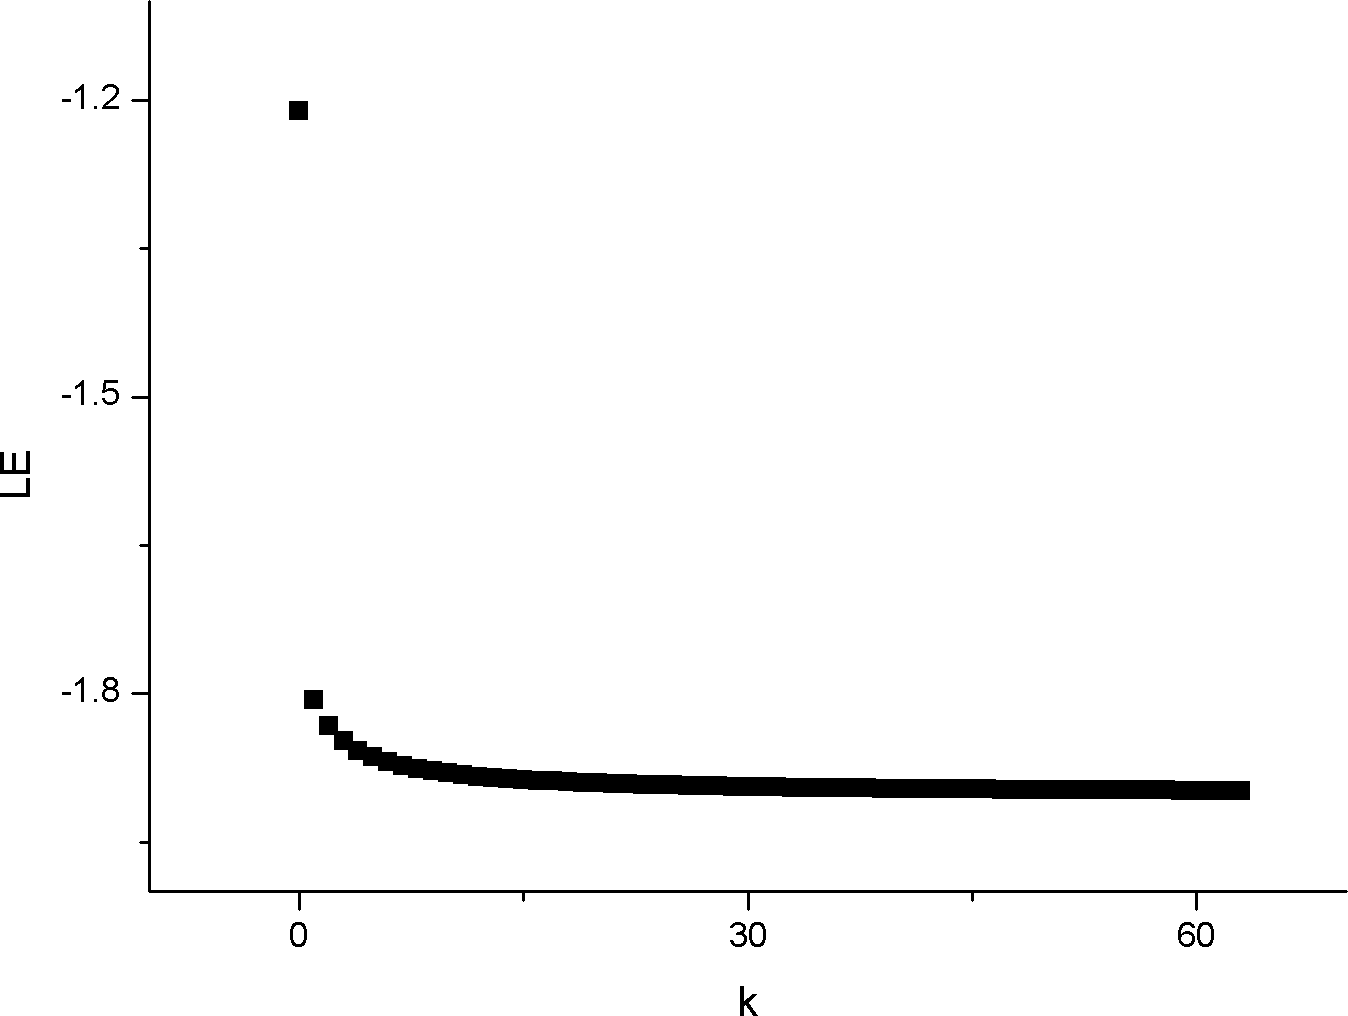
\includegraphics[width=8cm]{Lyapunovexpo_gq}
        \caption{\label{fig:1stWrongSpectrum}
        My first attempt at computing Lyapunov spectrum for $L=22$
        \KS\ system. Instead of $t\to\infty$ this is for $t\to 2$,
        much shorter than the shortest time scale of the system, so
        this is -at best- computation of the relaxation of initial
        tangent space vector mysteriously initialized as
        $\varPsi_k=(0,\cdots,0,k,0,\cdots,0)$.}
    \end{figure}

\item[2013-03-03 Predrag]
To help a bit with starting writing, I have edited your text (you can
see edits by using diff in Tortoise). Here is how you can
\QGedit{highlight your edits}, and here is how you can add a dated
footnote\QG{2013-03-03}{This is a footnote. Always enter the date, so
we know how old it is.}.

Always trim the figures: your Lyapunovexpo\_gq.png had lots of white
space around the edges.

\item[2013-03-03 Predrag]
Almost everything seems to go wrong in this approach of yours, but
now that you are writing (however tersely) we can start understanding
what the difficulties are. My guess is that you have not read this
entire blog, and have not studied the relevant \KS\
papers\rf{SCD07,Christiansen97}, so you are reinventing the wheel.
Everything that is written in these papers is there for a reason...

Graduate students are brave people who immediately jump into the deep
end of the pool, without any testing. Here are two 2\dmn\ maps, the
Lozi map (for $a=1.85, b=0.3$)
% \PC{need figure of Lozi strange attractor}
\bea
   x_{n+1} &=& 1-a |x_{n}|+ b y_n  \continue
   y_{n+1} &=& x_{n}
\,,
\label{e_lozi_def}
\eea
and the H\'enon map (for $a=1.4, b=0.3$; described at length in
\refchap{c-Henon})
\bea
    x_{n+1}&=&1-ax^2_n+b y_n
        \continue
    y_{n+1}&=& x_n
\,,
\label{eq2.1a}
\eea
for which fixed points are available analytically\rf{DasBuch} (for
the Lozi map all periodic points are available analytically). So see
what Floquet exponents (often incorrectly called `Lyapunov' exponents
) your program returns for \po s of these humble maps, and then for
ergodic trajectories, before running the programs on ergodic
trajectories in zillion dimensions.

If your programs only apply to continuous time flows (ODEs rather
than maps), ChaosBook\rf{DasBuch} has \eqva\ and \po s for 2\dmn\
Lorenz and R\"ossler flows, and Evangelos has lots of \rpo s for the
\cLe; make sure your programs work on small systems first.

\item[2013-03-14 Qi Ge]
I have found the key problem of Runge-Kutta method in simulation of
\refeq{expan}. There are linear terms with the coefficient with 4th
power of $k$. This will cause great stiffness of numerical simulation
as a multi-step simulation method. In order to switch off this
stiffness, I choose \(L = 96\) and took the cutoff number for Fourier
modes to be $N=32$, with a time step \(h = 0.000001\). I got a
relatively reasonable Lyapunov spectrum:
     \begin{figure}[H]
        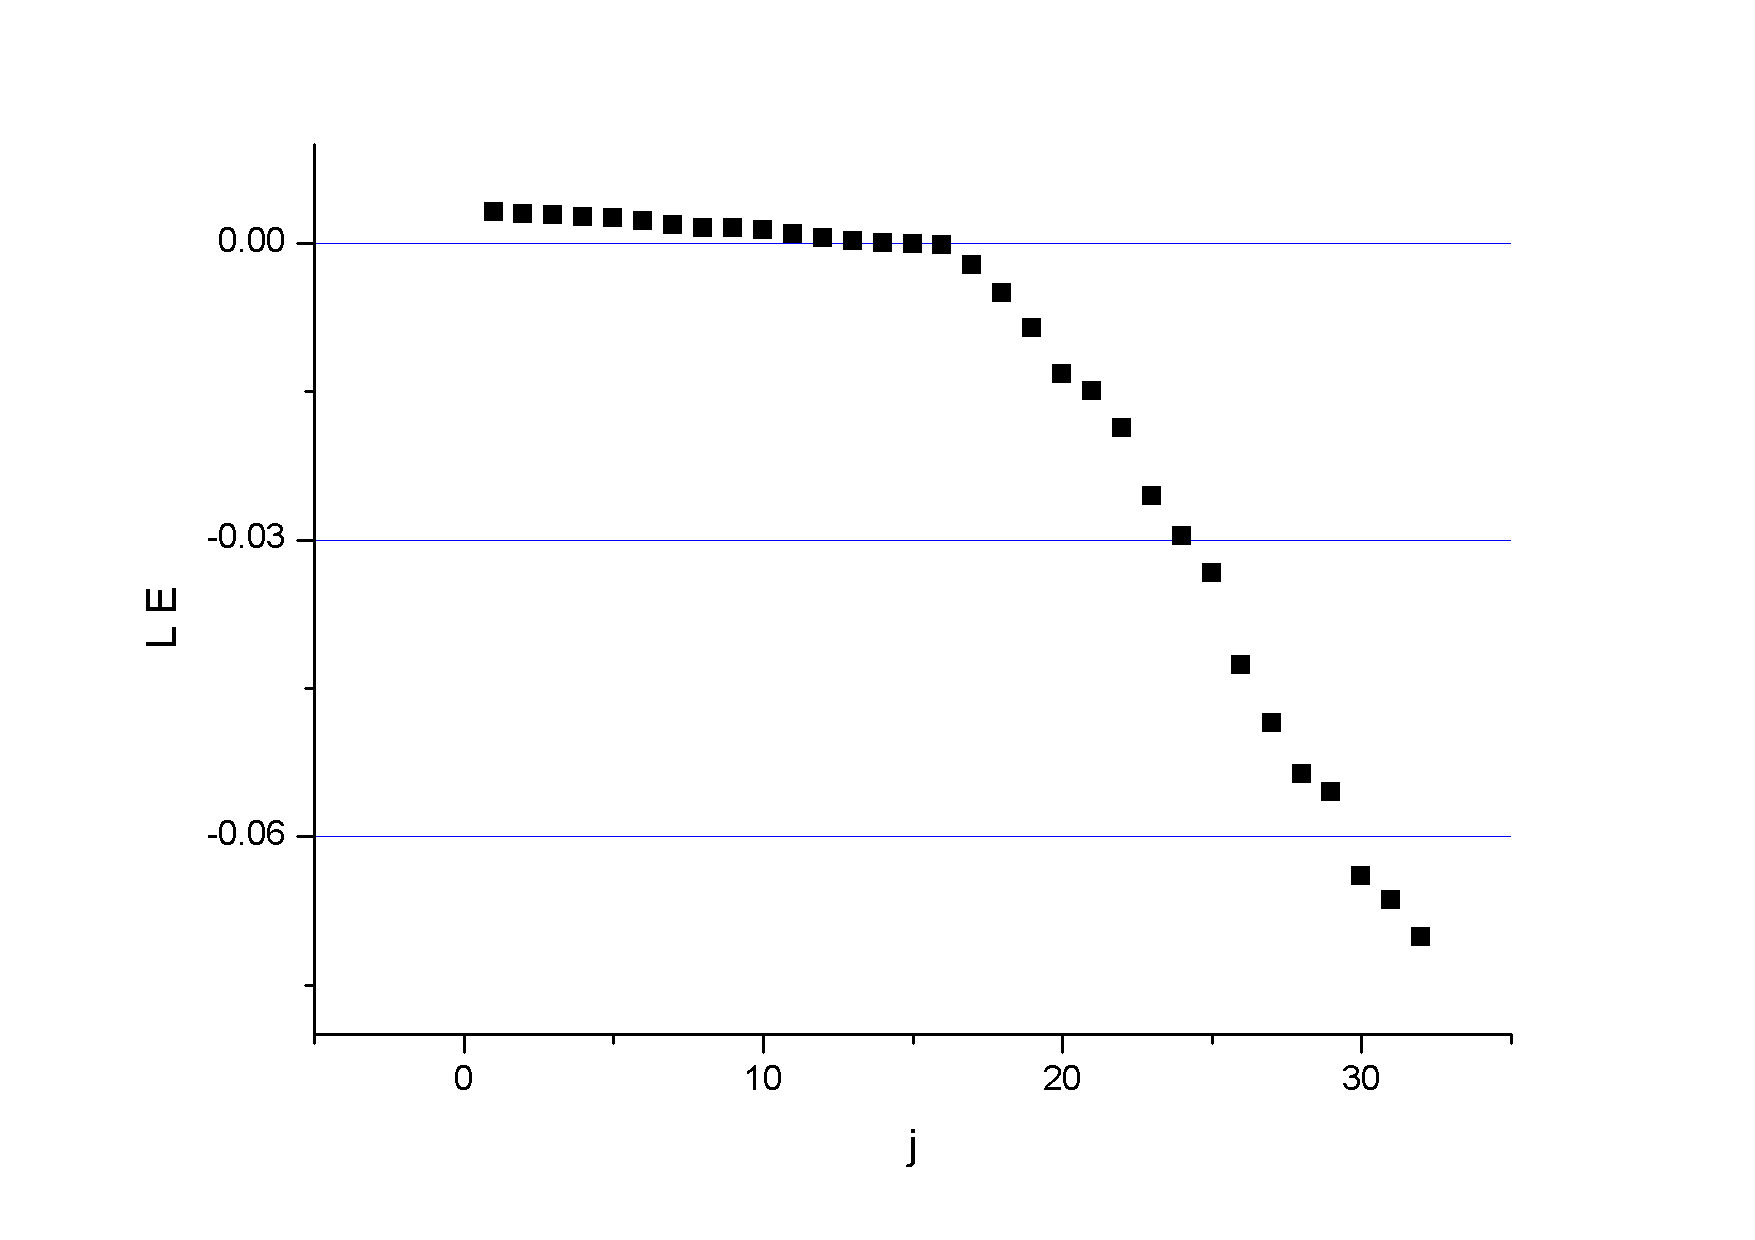
\includegraphics[width=8cm]{Lyapunovexpo_gq1.png}
        \caption{\label{Lyapunovexpo_gq1}
        Lyapunov spectrum with Runge-Kutta 4th order. $L = 96$,
        Fourier modes cutoff 32, time step $h = 0.000001$.}
    \end{figure}

However, I failed to get such a spectrum with \(L = 22\) and modes
number extends to 64.(which looks apparently wrong) I am currently
changing simulation into
\HREF{http://en.wikipedia.org/wiki/Linear_multistep_method\#Adams.E2.80.93Moulton_methods}
{Adam-Moulton} method, which is an one-step
simulation method.

\item[2013-03-14 Kazumasa to Qi Ge]
Yes, stiffness matters.
Implicit methods are common ways to overcome this problem,
 and that's why I used the Adams-Moulton method.
To further improve, it's better to split the linear and non-linear terms
 by the operator splitting method
 and use the implicit method only to the linear terms where the stiffness is.
I'm not saying that my algorithm is the best way to simulate the KS equation,
 but at least it's suited to practical use.

\item[2013-03-14 Ruslan to Qi Ge]
Or you can use the method developed by Cox and
Matthews\rf{cox02jcomp} and improved by Kassam and
Trefethen\rf{ks05com}, where the linear part is integrated exactly.
My Matlab code {\tt ksfmetd2.m} is based on this method and it is
stable and reasonably accurate with time step as large as 0.25.  It
also solves variational problem, so can be used to calculate Lyapunov
exponents.  See {\tt ksfmlyap.m} in {\tt siminos/matlab/ruslan/},
read {\tt 00ReadMe.txt}.  If you want to compute Lyapunov exponents
using the standard GS procedure, the relevant code is in {\tt
ksdupo.m} in the same folder (look for the cell "\%\% Compute
Lyapunov exponents of KS (using ksfmlyap and GS)").

\item[2013-02-19 Predrag]
% So far you have tweeted to the repository on March 13, 2, Feb 22:
% this is no 'minimum two' detailed write-ups per week. For example, I
% am not really sure that the version of \KS\ equation you are solving
% is the same as what we do. For the record, it should be what
I have now entered \KSe\ in your project report
\refsect{sect:introQG}, so one can compare to \refref{SCD07}. Form of
the equation matters, as Lyapunov exponents are dimensionally
1/[time], and units of time depend on the form of \KSe.


% \item[2013-02-19 Predrag]
%Regarding \reffig{Lyapunovexpo_gq1} - reread {\bf [2013-03-03
%Predrag]} above: ``Always trim the figures: your *.png had lots of
%white space around the edges.''

\item[2013-02-19 Predrag]
Regarding \reffig{Lyapunovexpo_gq1}: time step $h = 0.000001$ looks
very small to me; the shortest \po\ for $L = 22$ we have in
\refref{SCD07} has period $\period{p} = 16.3$, so simulations have to
be run for $10^2-10^4$ time units at least.
% I do not know what you
% did, as you give no indication
How long did you run the simulation?
Some exponents should be exactly zero (discussed earlier in the
blog): how many marginal exponents do you have, with what accuracy?

% ``A relatively reasonable Lyapunov spectrum''
Comparing with
\refFig{fig:lyapSpecRscld}\,(a): Neither the $j/L$ nor the
$\Lambda^{(j)}$ axis have your units. To me too many of your exponents
seem to be positive, so presumably you have not settled on the
attractor yet.

Please read {\bf 2009-09-14 Predrag} above: try to plot  $x$-axis in
$j/\tildeL = 2 \pi j/L$ units, as in \reffig{fig:lyapSpecRscld}.
Plotting it as a function of $j$ makes different $L$ simulations not
lie on the same plot.

Ruslan uses the same \KSe\ convention as Kassam and
Trefethen\refrefs{ks05com}. I have saved the Trefethen Matlab code
\HREF{http://chaosbook.org/extras/Trefethen/kursiv.m} {here}. Perhaps
you want to c++ it, see how it runs for you, or run it in Matlab and
compare with your code. There might be something else useful on
\HREF{http://chaosbook.org/extras/}{ChaosBook.org/extras} homepage,
for example the simulations by the spring 2007 GaTech chaos class.

Siminos has other codes, if needed, on a different repository. My own
\KS\ code is probably too antiquated to be worth your time.

\begin{verbatim}
 cd siminos/lyapunov/
 pdflatex blog; bibtex blog; pdflatex blog
\end{verbatim}

You can search the blog for 'Trefethen' for other discussions
(Kazumasa has reservations about the Trefethen\rf{ks05com} algorithm,
but Ruslan is OK with it).

A discussion of stiffness in integrating PDEs can be found
\HREF{http://www.pvv.ntnu.no/~berland/talks/berland05expintro.pdf}
{here}. \HREF{http://www.math.ntnu.no/num/expint/} {Here} is Matlab
package for testing 47 (!) schemes.

\item[2013-02-22 Predrag to Qi Ge]
I have written a new chapter in ChaosBook.org and copied it to
\refchap{c-Lyapunov} here, as a start of what needs to be written up
about your computation of Lyapunov spectra. It would be great if you
continued the exposition in your project report
\refsect{sect:introQG}. In the first draft, do not worry about
English -we'll help you with that-- just focus on the formulas. Write
down what a starting graduate student would need to know to be able
to set up the calculation.


\end{description}

\renewcommand{\ssp}{a}
